\documentclass[11pt]{article}
\usepackage[margin=1in]{geometry}
\usepackage{graphicx}
\usepackage{booktabs}
\usepackage{parskip}
\usepackage{enumitem}
\usepackage{titlesec}
\usepackage{xcolor}
\usepackage{hyperref}

\definecolor{e3blue}{HTML}{2A78D6}
\titleformat{\section}{\large\bfseries\color{e3blue}}{\thesection}{0.5em}{}
\titleformat{\subsection}{\normalsize\bfseries}{\thesubsection}{0.5em}{}

\title{\textbf{Q3: Forward-Looking Revenue Outlook \& Recommendation}\\
\large GCV Solar + Storage Valuation --- NYISO N.Y.C. Zone}
\author{E3 Applicant Exercise}
\date{2026}

\begin{document}
\maketitle

\section*{Q3a. How will each project's revenue stream evolve over the next decade, and why?}

\subsection*{Standalone Solar --- capture price likely erodes over time}
New York's Climate Leadership and Community Protection Act (CLCPA) mandates 70\% renewable
electricity by 2030 and a zero-emission grid by 2040, implying a large wave of new solar (and
offshore wind) entering NYISO downstate over the next decade. As more solar comes online, midday
supply floods the market and pushes midday prices down relative to the rest of the day --- the
``duck curve'' / solar cannibalization effect well documented in CAISO and emerging in NYISO.
Since this project only earns during daylight hours, its capture price (currently $\approx$100\%
of the flat average, per Q1b) should decline as a share of the market average even if the
\emph{overall} price level rises with electrification-driven demand growth.

\subsection*{Standalone Storage --- value likely increases over time}
The same trend that hurts solar helps storage: more solar depresses midday prices and steepens
the evening ramp (net load jumps sharply after sunset as solar drops off but demand stays high),
widening the daily price spread storage arbitrages. NYC's Peaker Rule is also retiring older
fossil peakers, tightening local capacity and likely increasing storage's importance (and
capacity-market value) for reliability. Countervailing risk: as more storage itself gets built to
chase this same spread, the arbitrage opportunity can compress again (``storage cannibalization'')
once the market saturates --- so the value increase is not indefinite.

\subsection*{Combined System --- the interaction benefit should grow}
Our Q2c finding (interaction $\approx$ +0.03\%) reflected minimal solar clipping today. As solar
penetration rises and mid-day curtailment risk increases system-wide, a co-located battery's
ability to absorb otherwise-clipped or negative-priced solar energy becomes more valuable --- so
the strategic case for pairing solar and storage should strengthen over the decade, even though
it is a weak argument today.

\section*{Q3b. Approach with 10 additional hours}

Priority-ordered by expected impact on the answer:

\begin{enumerate}[leftmargin=1.4em]
  \item \textbf{Forward price shapes ($\sim$3 hrs)} --- Replace the 2023 backcast with a
  forward-looking hourly price shape reflecting expected capacity additions/retirements and load
  growth (electrification of heating/EVs, data center demand). Use published NYISO planning
  studies / NYSERDA CLCPA outlooks as the fundamental driver rather than building a full
  production-cost model from scratch.
  \item \textbf{More realistic storage \& solar operating assumptions ($\sim$2 hrs)} --- Realistic
  round-trip efficiency ($\sim$85--90\%, not the given 100\%), solar degradation ($\sim$0.5\%/yr),
  battery degradation/augmentation schedule, and multi-cycle-per-day dispatch where economic.
  \item \textbf{Add capacity \& ancillary revenue streams ($\sim$2 hrs)} --- Energy arbitrage alone
  understates storage value; NYISO capacity market (ICAP) and frequency regulation are often the
  majority of a merchant battery's revenue stack today. This is likely the single biggest gap in
  our Q2 analysis.
  \item \textbf{Scenario/sensitivity analysis ($\sim$2 hrs)} --- Run high/low cases on load growth,
  gas prices, and renewable build-out pace rather than a single point forecast, given how uncertain
  the 10-year price path is.
  \item \textbf{Full pro forma ($\sim$1 hr)} --- Layer in the provided capex, O\&M, financing, and
  ITC/IRA tax credit treatment to get NPV/IRR rather than simple payback.
\end{enumerate}

\section*{Q3c. Recommendation}

Using simple payback (capex $\div$ 2023 backcast energy-only revenue, ignoring
financing/tax/O\&M --- a reasonable first screen given the time constraints):

\begin{table}[h!]
\centering
\begin{tabular}{lrrr}
\toprule
\textbf{Configuration} & \textbf{Capex} & \textbf{Annual Revenue} & \textbf{Simple Payback} \\
\midrule
Standalone Solar             & \$405M & \$18.9M & $\sim$21 yrs \\
Standalone Storage           & \$75M  & \$2.5M  & $\sim$30 yrs \\
\textbf{Combined Solar + Storage} & \textbf{\$445M} & \textbf{\$21.4M} & \textbf{$\sim$21 yrs} \\
\bottomrule
\end{tabular}
\end{table}

\begin{figure}[h!]
\centering
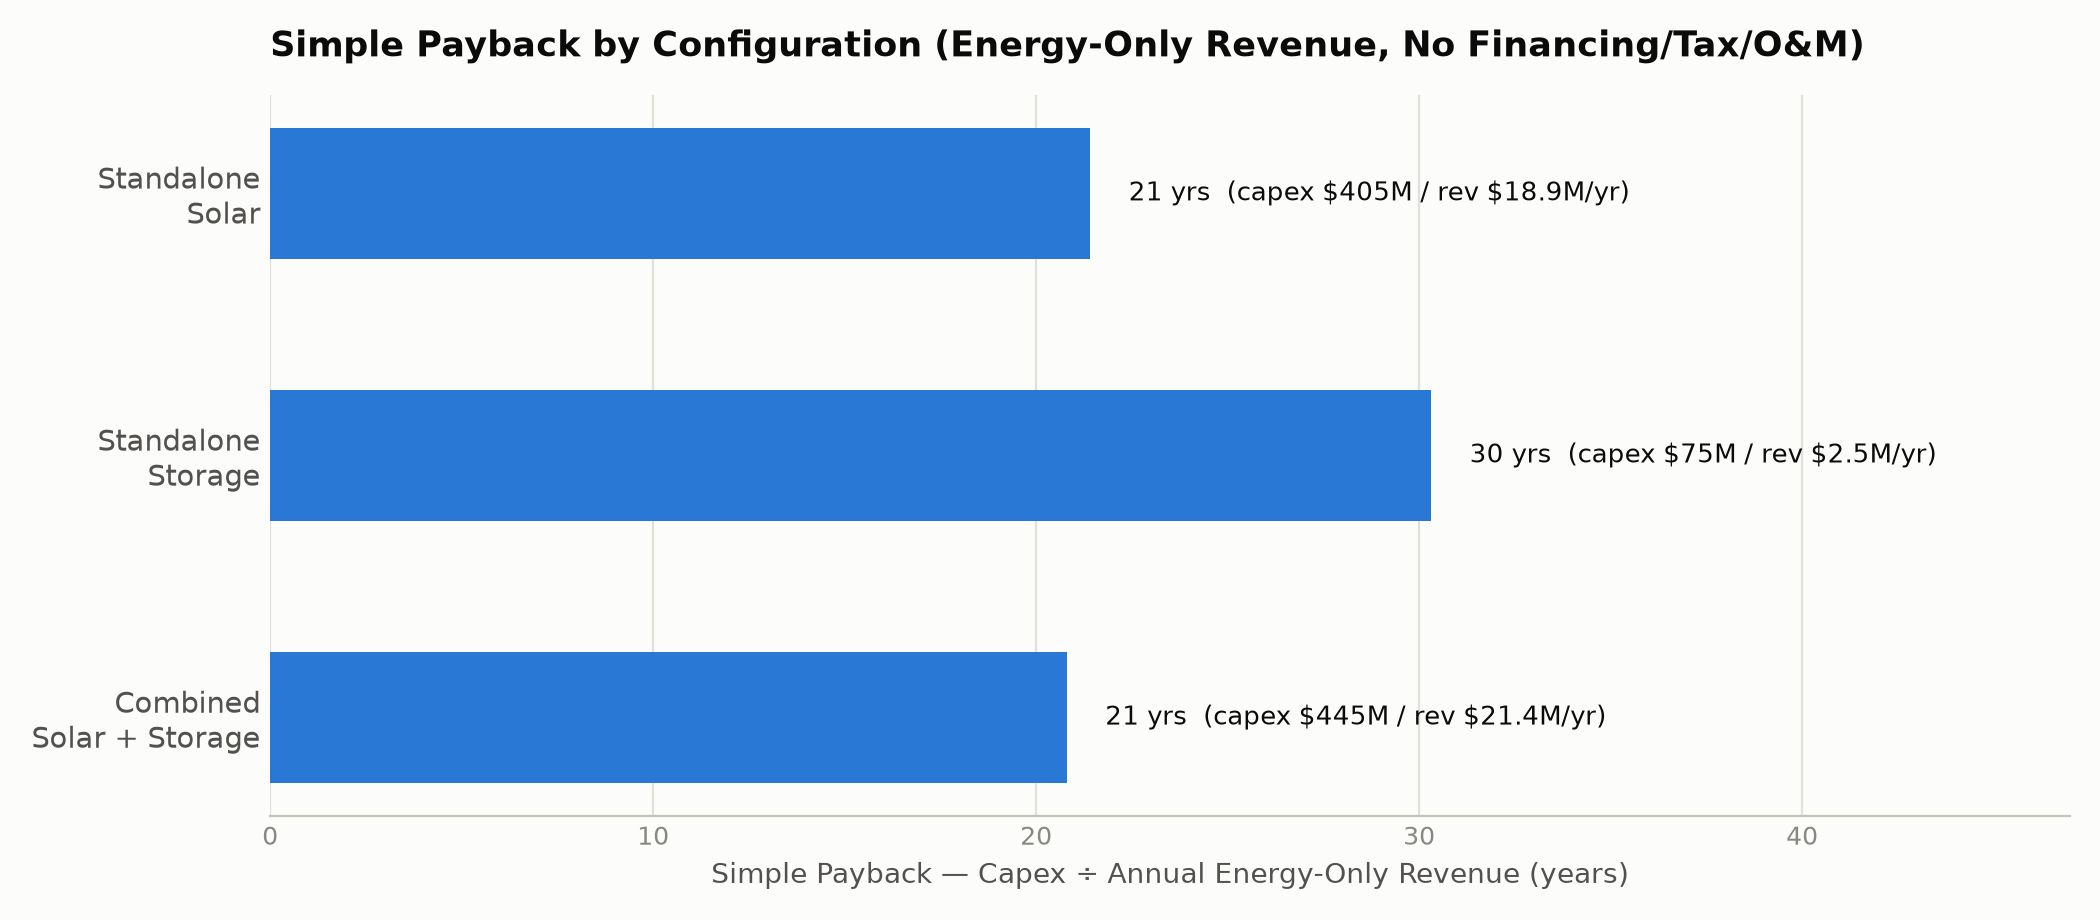
\includegraphics[width=\textwidth]{q3_payback_comparison.png}
\end{figure}

\textbf{Recommendation: the Combined Solar + Storage installation}, with moderate confidence,
for three reasons:

\begin{itemize}[leftmargin=1.4em]
  \item It matches standalone solar's payback almost exactly, so GCV isn't giving up economics
  to add storage.
  \item It is more capital-efficient than building the two technologies as separate projects: the
  combined package's per-unit equipment pricing (\$1.25/W solar, \$350/kWh storage) is cheaper
  than standalone pricing, saving \textbf{$\sim$\$35M in capex} for essentially the same revenue
  as running the two standalone projects side-by-side.
  \item It better hedges the Q3a trend: as solar capture prices likely erode over the decade,
  co-located storage is the piece of the portfolio whose value should be rising, partially
  offsetting that decline.
\end{itemize}

\textbf{Caveat:} standalone storage still looks weak here ($\sim$30-year payback) purely because
we have only modeled real-time energy arbitrage. Storage's real merchant revenue stack usually
includes capacity and ancillary services --- omitted here for time --- so this recommendation,
especially the case for the storage component, should be revisited once that analysis (Q3b, item 3)
is done before GCV commits capital.

\end{document}
